% arara: pdflatex: { options: ["--synctex=1"] }
% arara: biber if found('log', 'LaTeX Warning: There were undefined references.')
% arara: pdflatex: { synctex: yes } until !found('log', 'undefined references')

%%%
 % File: /main.tex
 % Created Date: Monday, May 6th 2024
 % Author: Zihan
 % -----
 % Last Modified: Thursday, 6th June 2024 1:58:30 pm
 % Modified By: the developer formerly known as Zihan at <wzh4464@gmail.com>
 % -----
 % HISTORY:
 % Date      		By   	Comments
 % ----------		------	---------------------------------------------------------
%%%

\documentclass[journal]{IEEEtran}
\usepackage{amsmath,amsfonts}
\usepackage{algorithmic}
\usepackage{algorithm}
\usepackage{array}
% \usepackage[caption=false,font=normalsize,labelfont=sf,textfont=sf]{subfig}
\usepackage{textcomp}
\usepackage{stfloats}
\usepackage{url}
\usepackage{verbatim}
\usepackage{graphicx}
% \usepackage{cite} % conflicts with biblatex
\usepackage{subcaption} % for subfigures
\usepackage{hyperref} % for hyperlinks
\usepackage{cleveref} % for \cref
\usepackage{doi}
% autocite
\usepackage{color}
\usepackage{csquotes}
% theorems
\usepackage{amsthm}
\newtheorem{theorem}{Theorem}
\newtheorem{lemma}{Lemma}
\newtheorem{definition}{Definition}
\newtheorem{assumption}{Assumption}

% Cref for lemma
\crefname{lemma}{lemma}{lemmas}
\Crefname{lemma}{Lemma}{Lemmas}
\crefname{assumption}{assumption}{assumptions}
\Crefname{assumption}{Assumption}{Assumptions}
\crefname{definition}{definition}{definitions}
\Crefname{definition}{Definition}{Definitions}

\hyphenation{op-tical net-works semi-conduc-tor IEEE-Xplore}

% image path: images/
\graphicspath{ {images/} }

% bibliography
\usepackage[backend=biber,style=ieee]{biblatex}
\bibliography{references}
% Suppress 'url' field in 'article' entries but keep 'doi'
\renewbibmacro*{doi+eprint+url}{%
  \iftoggle{bbx:doi}
    {\printfield{doi}} % keep doi
    {}%
  \iftoggle{bbx:eprint}
    {\usebibmacro{eprint}}
    {}%
  \iftoggle{bbx:url}
    {} % suppress url
    {}%
}
% Suppress 'isbn' field
\AtEveryBibitem{%
  % exclude 'isbn' field from all entries but books
  \ifentrytype{book}{}{\clearfield{isbn}}
}

% Suppress 'issn' field
\AtEveryBibitem{%
  \clearfield{issn}
}

% tables
\usepackage{booktabs}       % for professional tables
\usepackage{multirow}       % multirow in tables
\usepackage{threeparttable} % for table notes
\renewcommand{\cite}[1]{~\autocite{#1}}
\begin{document}

\title{\LARGE \bf Scalable Co-Clustering for Large-Scale Data through Dynamic Partitioning and Hierarchical Merging}

% The paper headers
% \markboth{Journal of \LaTeX\ Class Files,~Vol.~14, No.~8, August~2021}%
% {Shell \MakeLowercase{\textit{et al.}}: A Sample Article Using IEEEtran.cls for IEEE Journals}

% \IEEEpubid{0000--0000/00\$00.00~\copyright~2021 IEEE}
% Remember, if you use this you must call \IEEEpubidadjcol in the second
% column for its text to clear the IEEEpubid mark.
\author{}
\maketitle

\begin{abstract}
  Co-clustering algorithms are effective at uncovering complex multi-dimensional data patterns by concurrently grouping rows and columns. However, they are limited by scalability challenges and high computational complexity. This paper presents a novel and scalable co-clustering method designed to handle large-scale data efficiently. First, we propose a dynamic partitioning algorithm that divides large data matrices into smaller submatrices, facilitating parallel processing and significantly reducing computational and storage demands. The configurations of the submatrices are optimal based on a probabilistic model, guaranteeing convergence with iterations determined by the data matrix's scale. Besides, we develop a hierarchical co-cluster merging algorithm that iteratively combines co-clusters from submatrices, ensuring robust and consistent clustering performance. The proposed framework also supports integration with various co-clustering techniques and does not require specialized main thread performance, making it practical for real-world applications. Experimental evaluations demonstrate that our method outperforms existing solutions in scalability, efficiency, and co-cluster identification quality, particularly in high-dimensional and heterogeneous data scenarios. Specifically, our extensive evaluations show that \emph{MPHMCo} achieves substantial improvements, with a significant reduction in computation time—approximately 83\% for dense matrices and up to 30\% for sparse matrices.
\end{abstract}

\begin{IEEEkeywords}
  Co-clustering, scalable, distributed computing, dynamic partitioning, hierarchical merging.
\end{IEEEkeywords}

\section{Introduction}
\IEEEPARstart{R}{ecent} advancements in machine learning have significantly benefited from the use of large-scale datasets. Clustering, a fundamental unsupervised learning technique, plays an important role in the preprocessing of large-scale training data. By grouping similar data together, clustering enables refined feature recognition and intricate pattern analysis. Consequently, clustering diminishes noise during model training and improves data organization, significantly boosting both the efficiency and effectiveness of large-scale models\cite{raskutti2002CombiningClusteringCotraining, li2014ClusteringguidedSparseStructural, ghimatgar2018ImprovedFeatureSelection, li2023DistributedClusteringCooperative, bertsimas2020InterpretableClusteringOptimization}. However, traditional clustering algorithms\cite{lloyd1982LeastSquaresQuantization, arthur2007KmeansAdvantagesCareful, mclachlan1987MixtureModelsInference} treat all features of data uniformly and solely cluster either rows (samples) or columns (features), as shown in Figure \ref{fig:cluster}. This approach overlooks the potential multi-dimensional relationships within the data, thereby limiting its effectiveness in applications with complex multi-dimensional data patterns.

\textit{Co-clustering}\cite{cheng2000BiclusteringExpressionData, kluger2003SpectralBiclusteringMicroarray, yan2017CoclusteringMultidimensionalBig} address these limitations by simultaneously grouping rows (samples) and columns (features), as shown in Figure \ref{fig:cocluster}. Co-clustering enables a more nuanced analysis of interdependencies between different data dimensions, uncovering complex correlations between diverse data types. This approach is especially important in scenarios where the relationships between rows and columns are as important as the individual entities themselves. For example, in bioinformatics, co-clustering can identify gene-related patterns leading to biological insights by concurrently analyzing genes and conditions\cite{higham2007SpectralClusteringIts, kluger2003SpectralBiclusteringMicroarray, madeira2004BiclusteringAlgorithmsBiological, zhao2012BiclusteringAnalysisPattern, golchev2015BiclusteringAnalysisGene}.
In multimodal learning, co-clustering can integrate and analyze different types of data modalities, such as text and images, to reveal intricate connections and improve predictive performance across diverse datasets\cite{mu2022LearningHybridBehavior}.


\begin{figure}[t]
  \centering
  \begin{subfigure}[b]{0.22\textwidth}
    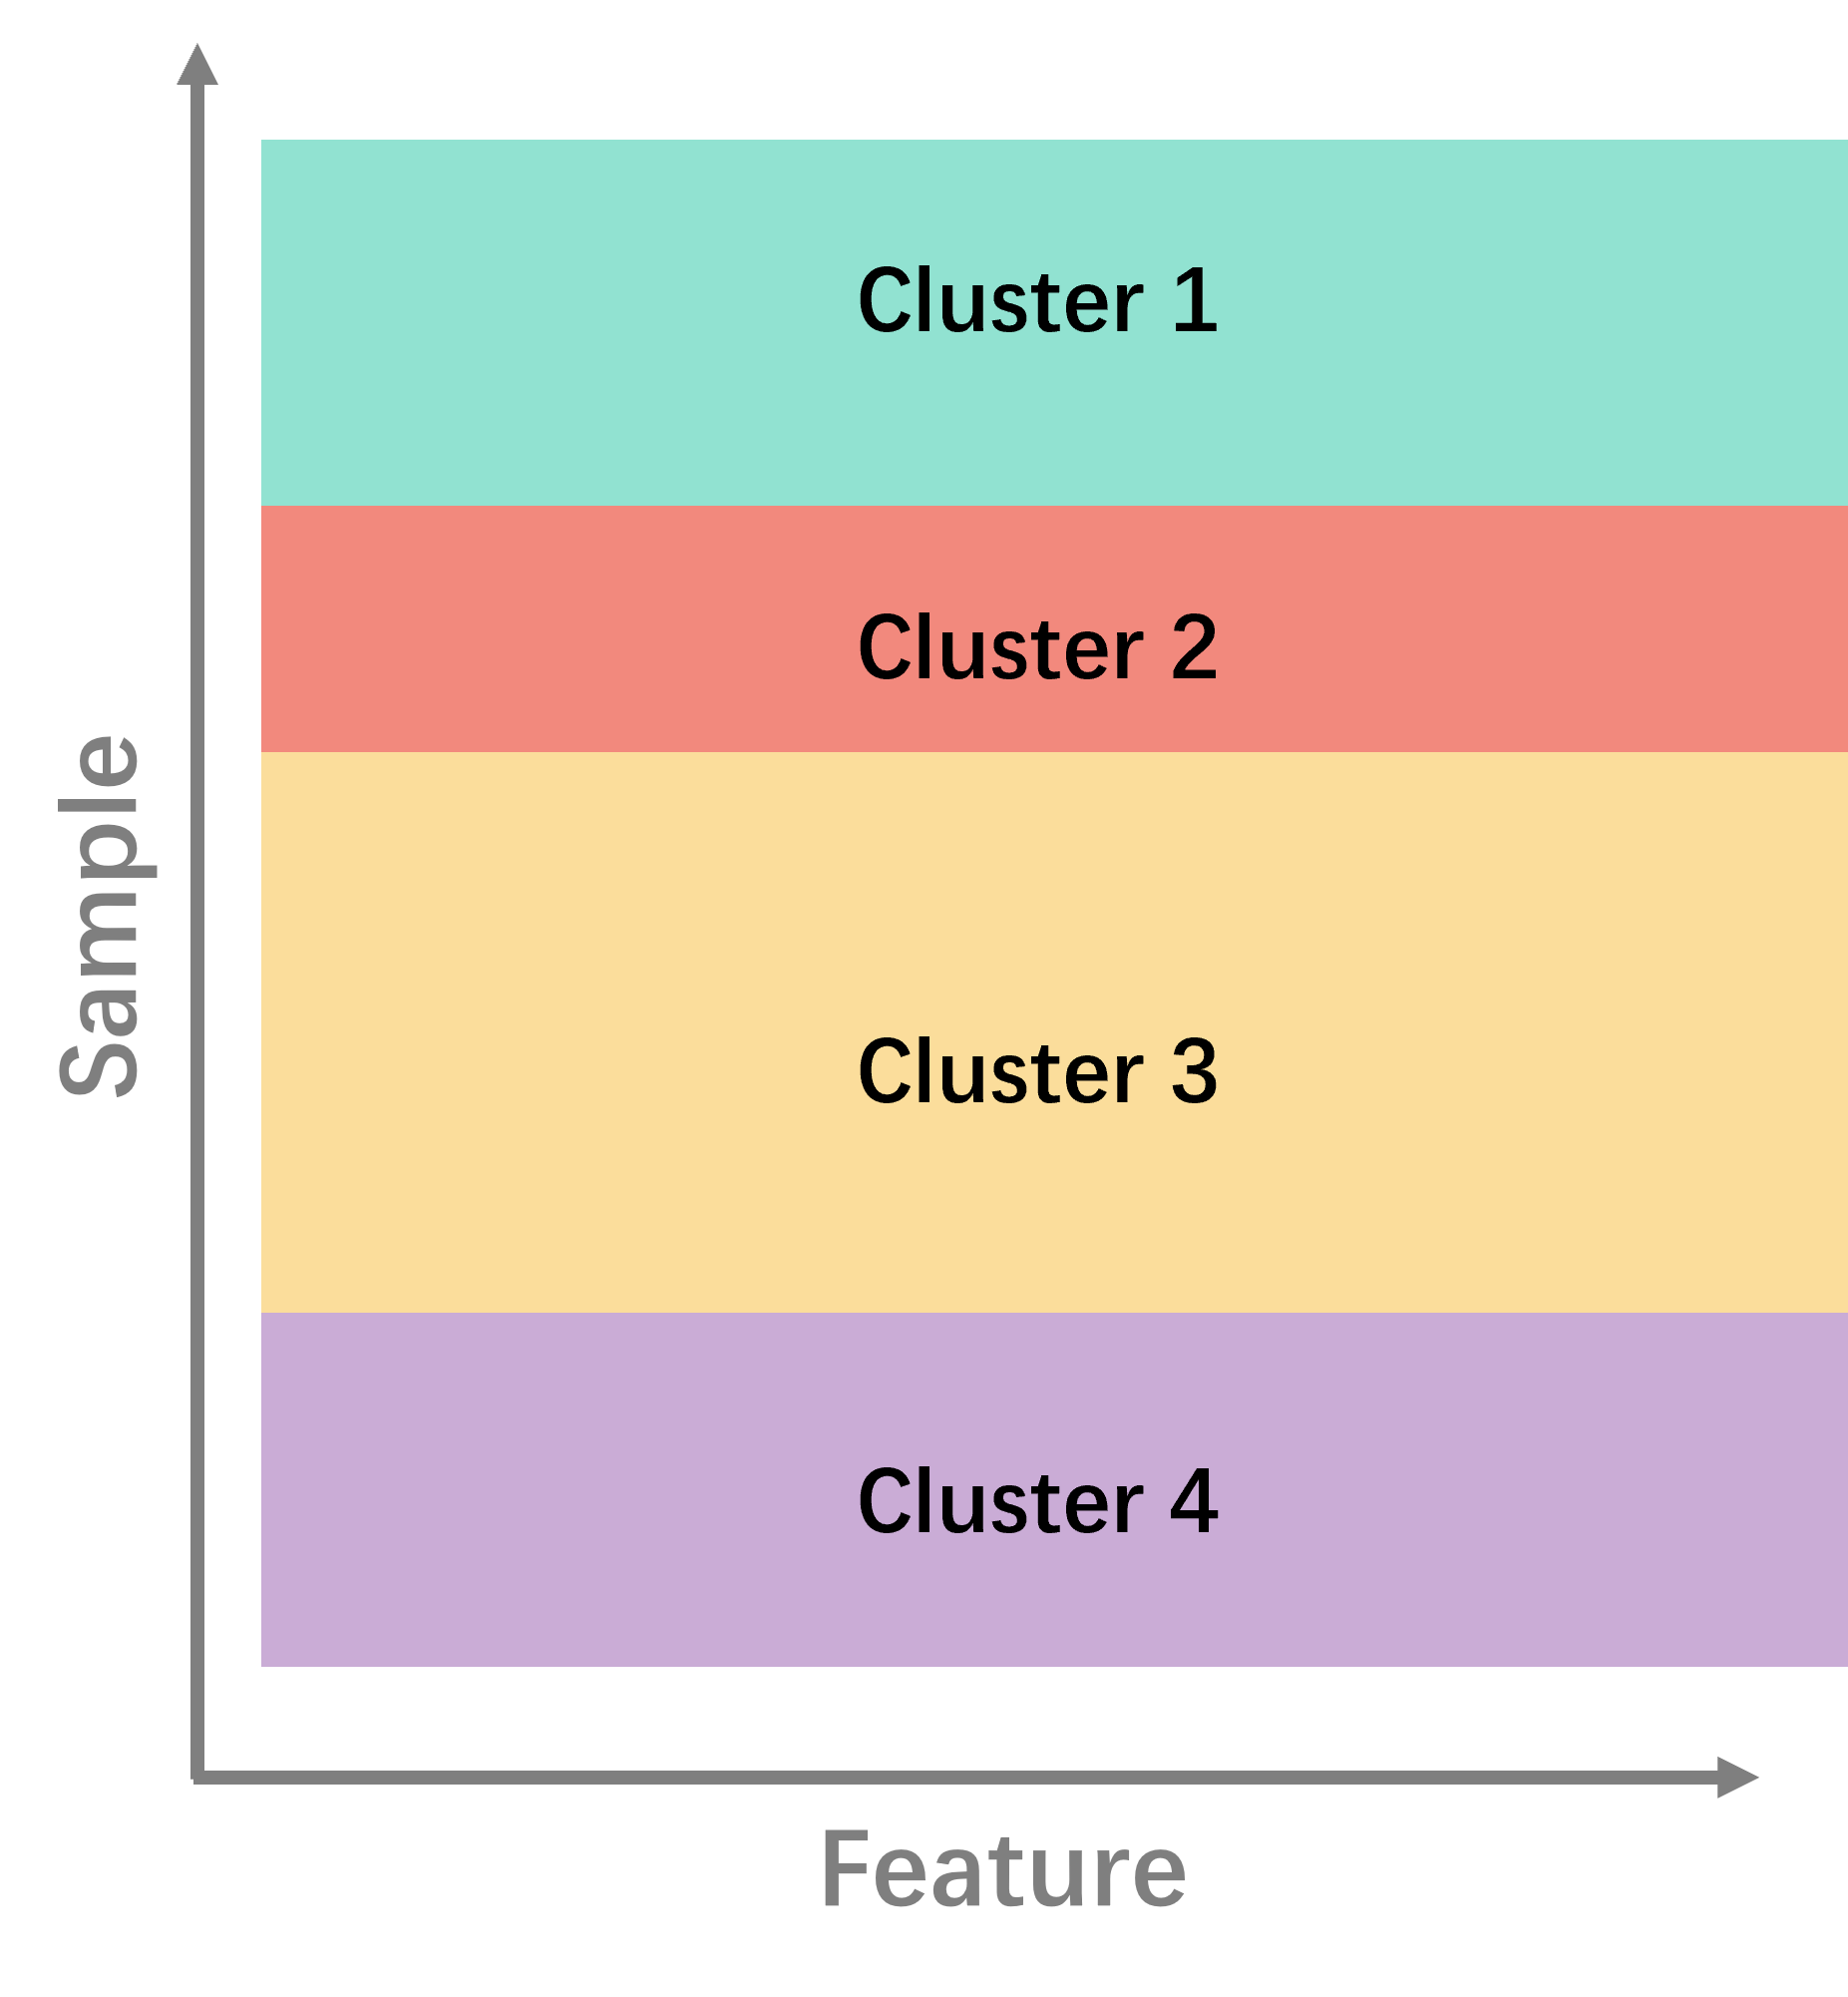
\includegraphics[width=\linewidth]{cluster.png}
    \caption{Clustering}
    \label{fig:cluster}
  \end{subfigure}
  \hfill
  \begin{subfigure}[b]{0.22\textwidth}
    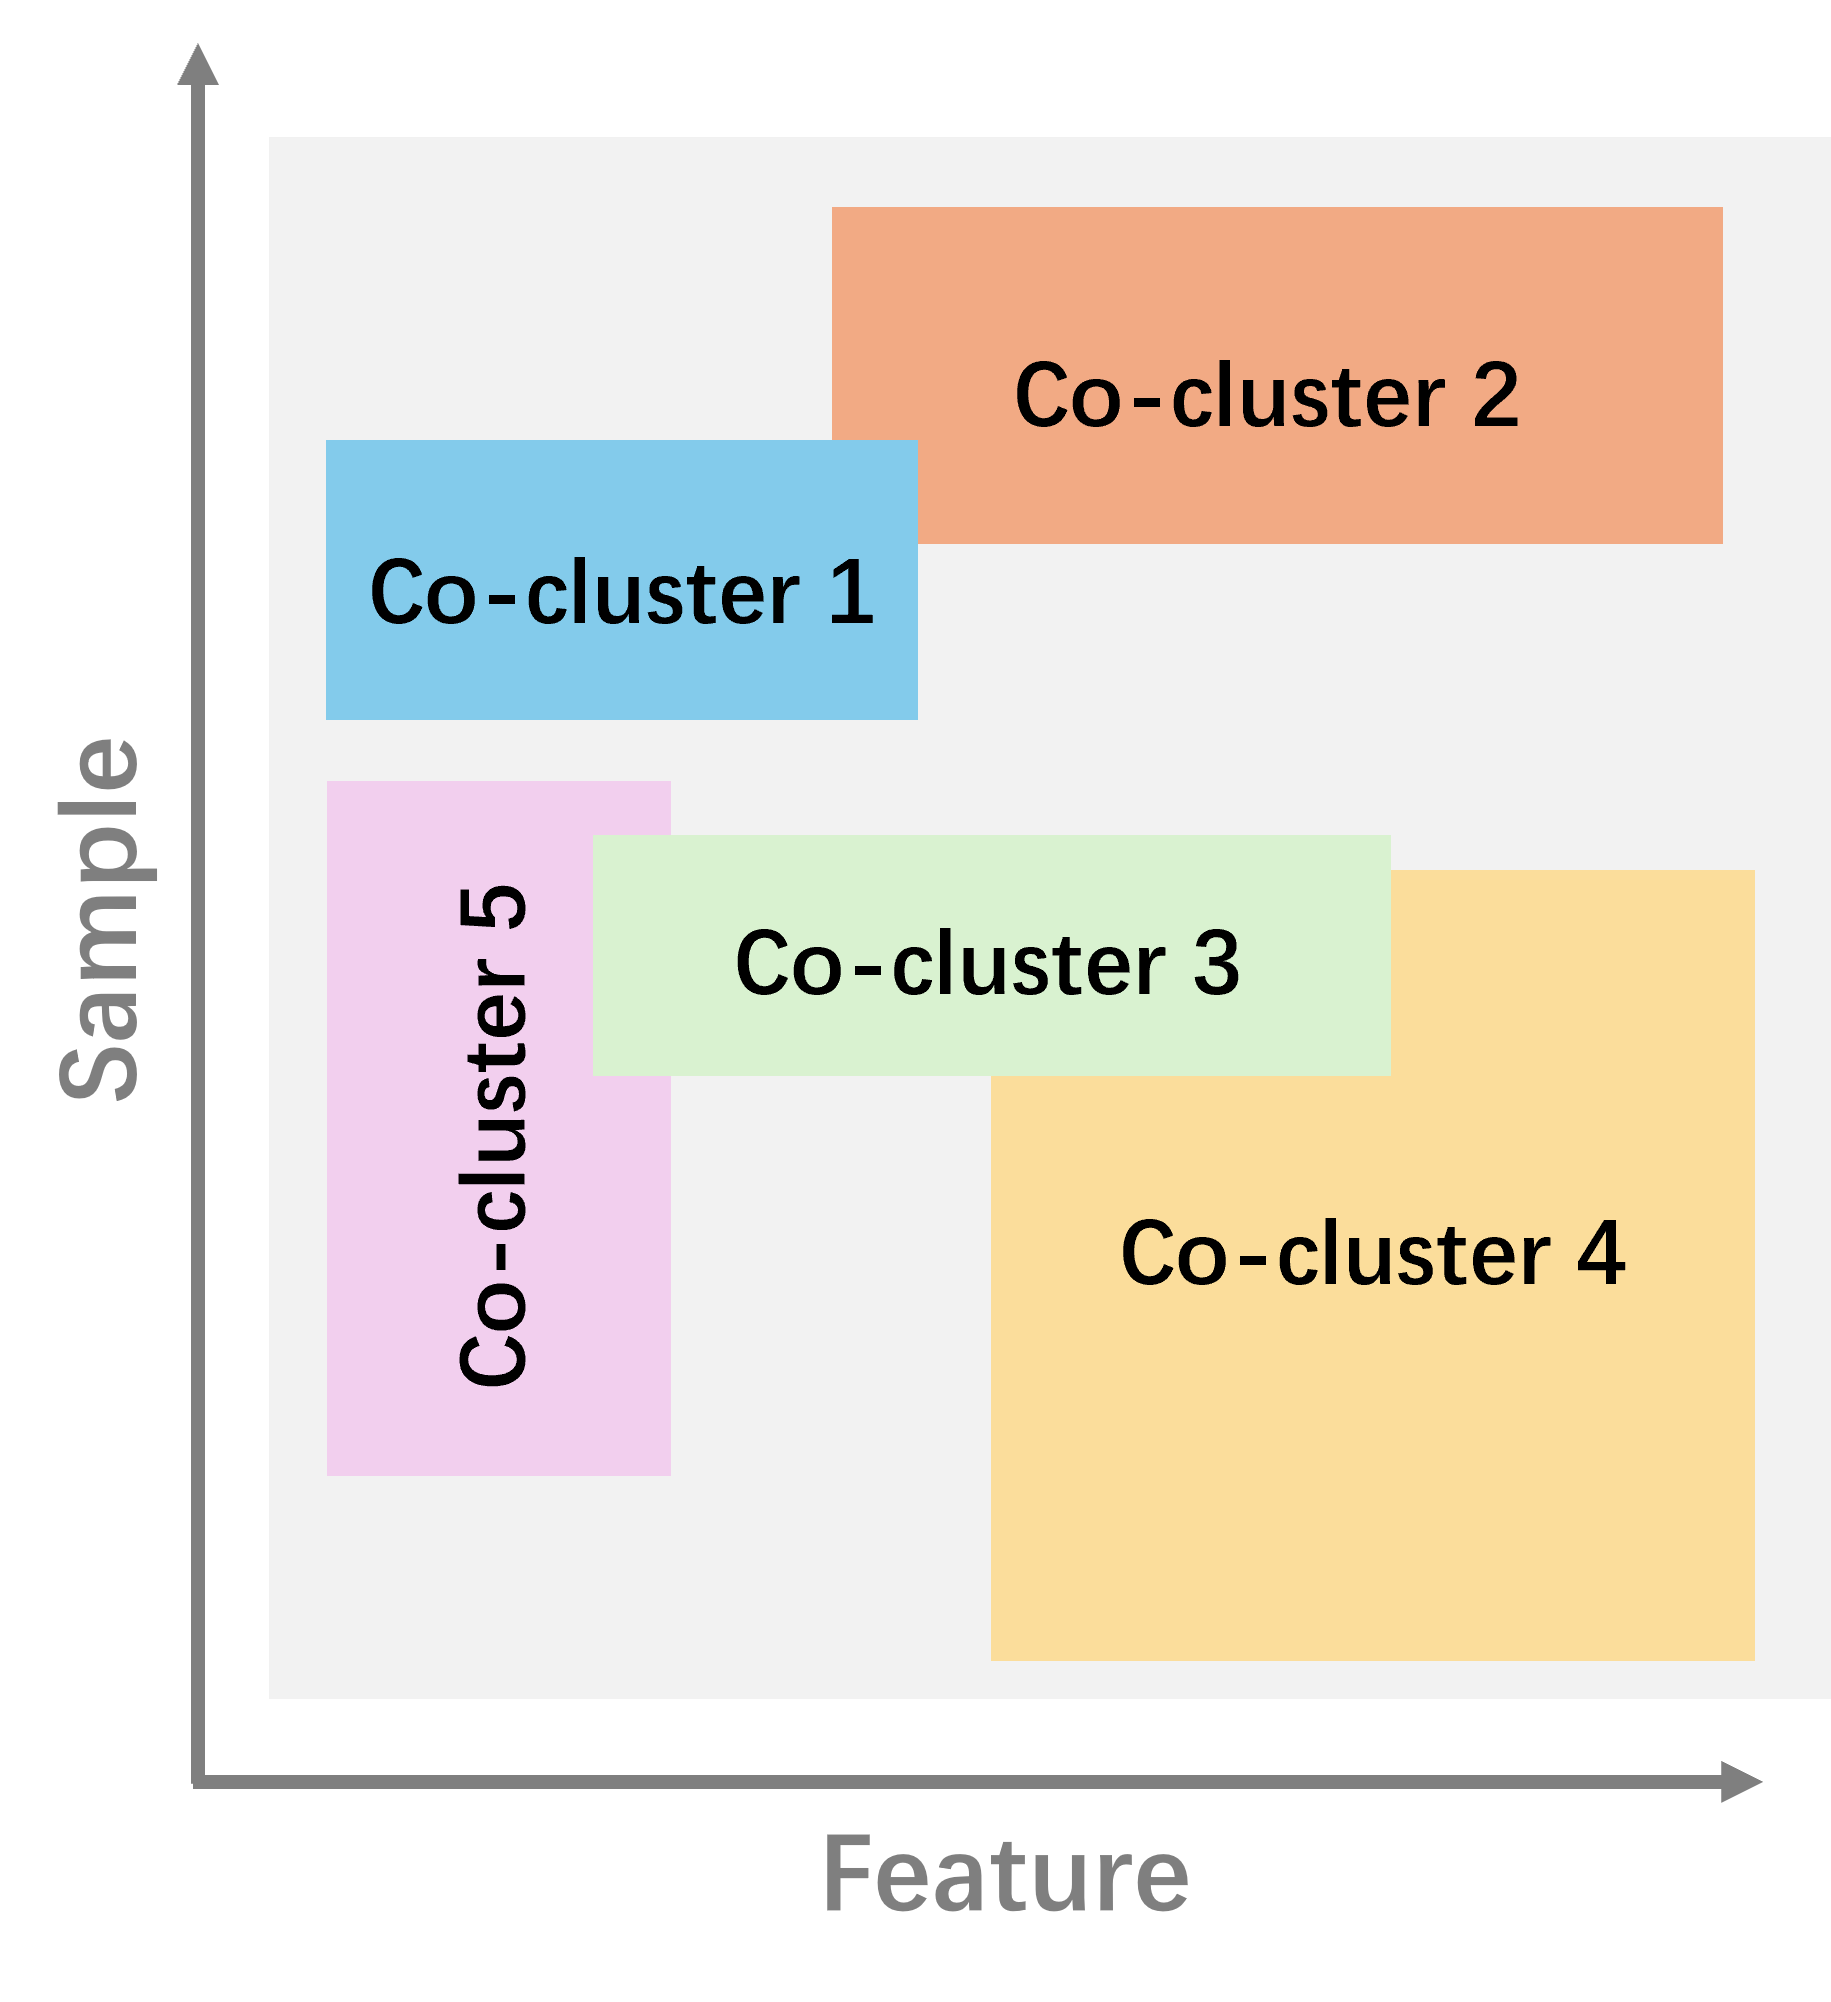
\includegraphics[width=\linewidth]{coc.png}
    \caption{Co-clustering}
    \label{fig:cocluster}
  \end{subfigure}
  \caption{An illustration of the differences between (a) Clustering and (b) Co-clustering.}
  \label{fig:cocomparison}
\end{figure}

While co-clustering has great potential, existing co-clustering algorithms are impractical for handling large-scale data due to scalability and high complexity issues\cite{cheng2015CoClusterDDistributedFramework}. This complexity arises from the need to simultaneously optimize both row and column clusters,  turning the problem into a multi-objective optimization task. This task involves minimizing multiple loss functions concurrently, often resulting in conflicting gradients and optimization paths. These conflicts complicate the convergence process, making it difficult to achieve efficient and effective clustering \cite{coello2007EvolutionaryAlgorithmsSolving}. To address these scalability limitations, PNMTF\cite{chen2023ParallelNonNegativeMatrix} employs parallelization using distributed computing frameworks. However, it lacks guaranteed iteration numbers and requires broadcasting a non-adaptive scale matrix, which limits its scalability. Similarly, Co-ClusterD\cite{cheng2015CoClusterDDistributedFramework}'s main thread must handle co-cluster statistics \(S_{cc}\), constraining its scalability. Despite attempts to distribute tasks, both algorithms still rely on the main thread to manage high-complexity tasks.

% \textit{Co-clustering}\cite{cheng2000BiclusteringExpressionData, kluger2003SpectralBiclusteringMicroarray, yan2017CoclusteringMultidimensionalBig} is a powerful technique in the field of unsupervised learning. Easier access to large-scale data has led to an increasing demand for scalable co-clustering algorithms in various applications, such as text mining\cite{fettal2024BoostingSubspaceCoclustering, chen2023ParallelNonnegativeMatrix, chen2023FastFlexibleBipartite, cheng2015Co-ClusterDDistributedFramework, song2013ConstrainedTextCoclustering, chen2010NonnegativeMatrixFactorization}, bioinformatics\cite{yu2021CoClusteringEnsemblesBased, huang2020CombiningBiclusteringMining, wang2019DualHypergraphRegularized, yang2011FindingCorrelatedBiclusters}, and recommendation systems\cite{dhillon2003InformationtheoreticCoclustering,li2021NovelCollaborativeFiltering, leung2011CLRCollaborativeLocation,he2024CoclusteringFederatedRecommender}.

To address these challenges, we propose a novel and scalable co-clustering method that is efficient and effective for large-scale data. Our method includes two core designs: a \textit{dynamic partitioning algorithm} and a \textit{hierarchical co-cluster merging algorithm}.
The proposed co-clustering method begins with our dynamic partitioning algorithm that divides the original data matrix into smaller submatrices. This partitioning facilitates parallel processing of co-clustering tasks across submatrices, significantly reducing both processing time and computational and storage demands for each processing unit. Our designed probabilistic model can determine the optimal number and configuration of these submatrices, ensuring comprehensive data coverage. If the atom co-clustering method is effective, this model guarantees that the entire framework will converge with an iteration number specified only by the scale of the data matrix, providing confidence in the robustness and reliability of our approach across diverse datasets.

Then, our hierarchical co-cluster merging algorithm iteratively combines the co-clusters from these submatrices. This process enhances the accuracy and reliability of the final co-clustering results and ensures robust and consistent clustering performance, particularly addressing issues of heterogeneity and model uncertainty. By leveraging a hierarchical merging strategy, we can efficiently integrate co-clusters without overwhelming any single processing unit, thereby maintaining scalability. Our method is modular, allowing any co-clustering method, including those with existing parallel designs, to be integrated seamlessly. This flexibility ensures that our approach can adapt and evolve with advancements in co-clustering techniques.

Our proposed method also includes a Message Passing Interface (MPI) implementation, which allows for effective distribution of the computational load across multiple nodes. The main computation node only needs to compute thresholds based on the size of the matrix, without requiring specialized performance beyond that of other nodes, making our approach more practical and scalable for large-scale applications. Unlike existing methods that require a high-performance central processing unit, our approach does not demand a supercomputer for the main thread. Additionally, our framework is probabilistically guaranteed to work.

The main contributions of this paper are as follows:
\begin{enumerate}
  \item \textbf{Dynamic Partitioning Algorithm:}
        We propose a dynamic partitioning algorithm grounded in our probabilistic model to determine the optimal parameters for dividing large matrices. This algorithm enhances parallel processing and reduces computational complexity.

  \item \textbf{Hierarchical Merging Algorithm:}
        We introduce a hierarchical merging algorithm designed to amalgamate co-clusters from submatrices. This method fortifies the co-clustering process, ensuring robustness and preserving data integrity.

  \item \textbf{MPI Implementation and Performance Evaluation:}
        We implement our algorithm using MPI (Message Passing Interface) and conduct extensive performance evaluations on large datasets. The results demonstrate significant improvements in computational efficiency and robustness.

\end{enumerate}

The remainder of this paper is organized as follows. Section \ref{sec:related_work} discusses related work in the field of co-clustering and parallel computing. Section \ref{sec:formula} presents the mathematical formulation and problem statement of co-clustering. Section \ref{sec:method} details our proposed scalable co-clustering method.
Section \ref{sec:analysis} focuses on the complexity analysis and probabilistic guarantees of our method.
Section \ref{sec:experiment} presents the experimental evaluation of our method. Finally, Section \ref{sec:conclusion} concludes the paper and outlines future research directions.

\section{Related work}
\label{sec:related_work}
\subsection{Co-clustering Models}

The concept of \emph{biclustering}, where both the rows and columns of data are clustered simultaneously, was first introduced by Hartigan \cite{hartigan1972DirectClusteringData} to analyze gene expression data. This pioneering approach recognized the importance of simultaneously considering multiple dimensions of data to uncover more nuanced patterns. Since then, biclustering has expanded to various other areas, giving rise to the broader concept of \emph{co-clustering}, which has led to the development of several models designed to address a range of analytical challenges.

Spectral Co-clustering with Singular Value Decomposition (SVD), introduced by Dhillon \textit{et al.} \cite{dhillon2001CoclusteringDocumentsWords}, became widely adopted due to its straightforward implementation and effectiveness. This method leverages the mathematical properties of SVD to identify clusters by analyzing the principal components of the data matrix. Spectral co-clustering has since become a foundational technique, inspiring two main branches in co-clustering research: graph-based and matrix factorization-based approaches.

The most widely used graph-based co-clustering method is the Flexible Bipartite Graph Co-clustering (FBGPC) \cite{chen2023FastFlexibleBipartitea}. FBGPC applies a flexible bipartite graph model directly to the original data, allowing for the simultaneous clustering of two distinct sets of objects, such as users and items in a recommendation system. This approach effectively captures the interactions between these sets, providing deeper insights into their relationships.

In contrast, Non-negative Matrix Tri-Factorization (NMTF) \cite{long2005CoclusteringBlockValue} represents a leading matrix factorization-based method. NMTF decomposes the data matrix into multiple non-negative matrices, which correspond to the underlying factors of the data. By independently clustering both samples and features, NMTF reveals the latent structures within the data. This method has proven to be particularly useful in applications where the interpretability of factors is crucial, such as bioinformatics and social network analysis. Our method is orthogonal to NMTF, allowing for potential integration to enhance co-clustering efficiency.

Another innovative method, Deep Co-Clustering (DeepCC) \cite{dongkuanxu2019DeepCoClustering}, combines the power of deep learning with traditional clustering techniques. DeepCC integrates deep autoencoders with Gaussian Mixture Models to improve the clustering of complex data. The autoencoders reduce the dimensionality of the data while preserving essential features, and the Gaussian Mixture Models identify clusters within this reduced space. Despite its advancements, DeepCC struggles with computational efficiency, particularly with diverse data types and iterative processes dependent on data sparsity. The deep learning components introduce additional layers of computation, which can be resource-intensive and time-consuming.

\subsection{Parallelizing Co-clustering}

To address the significant computational challenges posed by big data, parallel co-clustering methods have emerged as a vital solution. Parallelization leverages distributed computing frameworks to divide the computational load across multiple processors or machines, thereby improving scalability and efficiency.

Cheng \textit{et al.} \cite{cheng2015CoClusterDDistributedFramework} introduced a distributed co-clustering framework, Co-ClusterD, which utilizes an Alternating Minimization Co-clustering (AMCC) algorithm with sequential updates. Co-ClusterD partitions the data into smaller chunks, which are processed in parallel, and then combines the results. However, this method faces challenges with guaranteed convergence. The iterative nature of AMCC, coupled with the need for sequential updates, can lead to inefficiencies and bottlenecks, particularly as the size and complexity of the data increase.

While matrix factorization techniques have shown promise for co-clustering large datasets, scaling these algorithms for massive high-dimensional data remains an open challenge. Chen \textit{et al.} \cite{chen2023ParallelNonNegativeMatrix} proposed a parallel non-negative matrix tri-factorization (PNMTF) method that distributes computation across multiple nodes to accelerate factorizations. PNMTF decomposes the original matrix into simpler, non-negative components, which are then processed in parallel. However, even these advanced methods encounter difficulties with extremely large datasets. The need to broadcast intermediate results and synchronize updates across nodes introduces significant communication overhead, which can negate the benefits of parallelization.

Existing co-clustering algorithms\cite{chen2023ParallelNonNegativeMatrix, cheng2015CoClusterDDistributedFramework} rely on a central processing thread to handle complex tasks like managing co-cluster statistics. This centralization creates a bottleneck, significantly limiting their scalability and making them impractical for large-scale datasets. Additionally, the dual-focus analysis of co-clustering, which simultaneously optimizes row and column clusters, requires evaluating a vast number of potential relationships. This complexity can grow exponentially with the size of the data, making it impractical for large-scale applications.

In contrast, our proposed method adopts a divide-and-conquer strategy to overcome these limitations. By partitioning the input matrix into smaller submatrices, we reduce the dimensionality of each individual task, making them more manageable. Each submatrix is co-clustered in parallel, leveraging distributed computing resources to expedite the process. This technique reduces the complexity imposed by high dimensionality and minimizes the communication overhead associated with broadcasting and synchronization. The separate co-clustering results from each submatrix are then combined using a hierarchical merging algorithm to form the final co-clusters. This novel approach addresses the computational challenges inherent in co-clustering large-scale data and introduces a scalable solution tailored for big data.

\section{Mathematical Formulation and Problem Statement}\label{sec:formula}


\subsection{Mathematical Formulation of Co-clustering}
Co-clustering is a method designed to simultaneously group a set of rows and columns in a data matrix $\mathbf{A} \in \mathbb{R}^{M \times N}$, where $M$ denotes the number of features or variables and $N$ denotes the number of samples or objects. Each element $a_{ij}$ in the matrix at the $(i, j)$-th position represents the relationship or measurement between the $i$-th feature and the $j$-th object. The primary goal of co-clustering is to identify subsets of rows ($I$) and columns ($J$) into homogenous submatrices, $\mathbf{A}_{I, J}$, that exhibit distinctive patterns or uniform characteristics, thus forming coherent co-clusters. The objective is to partition $\mathbf{A}$ into $k$ row clusters and $d$ column clusters, resulting in $k \times d$ distinct co-clusters.

When rows and columns are optimally reordered, $\mathbf{A}$ can be visualized as a block-diagonal matrix, where each block represents a co-cluster with higher similarity within than between blocks. We define the row and column label sets as \( u \in \{1,\dots,k\}^M \) and \( v \in \{1,\dots,d\}^N \), respectively. Indicator matrices \( R \in \mathbb{R}^{M \times k} \) and \( C \in \mathbb{R}^{N \times d} \) are used to assign rows and columns to clusters, with the constraints \( \sum_k R_{i,k} = 1 \) and \( \sum_d C_{j,d} = 1 \), ensuring each row and column is assigned to exactly one cluster.

To evaluate if a submatrix $\mathbf{A}_{I, J}$ forms a coherent co-cluster, we define a score function \( f(\mathbf{A}_{I, J}) \) that quantifies the homogeneity of the submatrix.

\begin{definition}[Co-cluster Score Function]
  \label{def:co_cluster}
  Given a matrix $\mathbf{A} \in \mathbb{R}^{M \times N}$, $I$ and $J$ are the row and column indices of a submatrix $\mathbf{A}_{I, J}$. The co-cluster score function is defined as below:
  \begin{itemize}
    \item For a given submatrix $\mathbf{A}_{I, J}$, the co-cluster score function is defined as
          $$s(\mathbf{A}_{I, J}) = \frac{s_1}{s_2}. $$ where $s_1$ is largest singular value of $\mathbf{A}_{I, J}$ and $s_2$ is the second largest singular value of $\mathbf{A}_{I, J}$.
    \item For a given submatrix $\mathbf{A}_{I, J}$, the normalized co-cluster score function is defined as
          $$S(\mathbf{A}_{I, J}) = \frac{s(\mathbf{A}_{I, J})}{||\mathbf{A}_{I, J}||_F} $$ where $||\mathbf{A}_{I, J}||_F$ is the Frobenius norm of $\mathbf{A}_{I, J}$.
  \end{itemize}
\end{definition}

\subsection{Problem Statement}
This paper aims to develop a method that efficiently and accurately identifies co-clusters $\mathbf{A}_{I, J}$ within a matrix $\mathbf{A}$ representing large datasets. These co-clusters should exhibit specific structural patterns such as uniformity across elements, consistency along rows or columns, or patterns demonstrating additive or multiplicative coherence. Properly identifying and categorizing these patterns is crucial for understanding the complex data structures inherent in large datasets. This method is intended to improve the detection capabilities of co-clustering, enhancing both the efficiency and precision necessary for handling large-scale data challenges.

\section{The Scalable Co-clustering Method}
\label{sec:method}
\subsection{Overview}

\begin{figure*}[htbp]
  \centering
  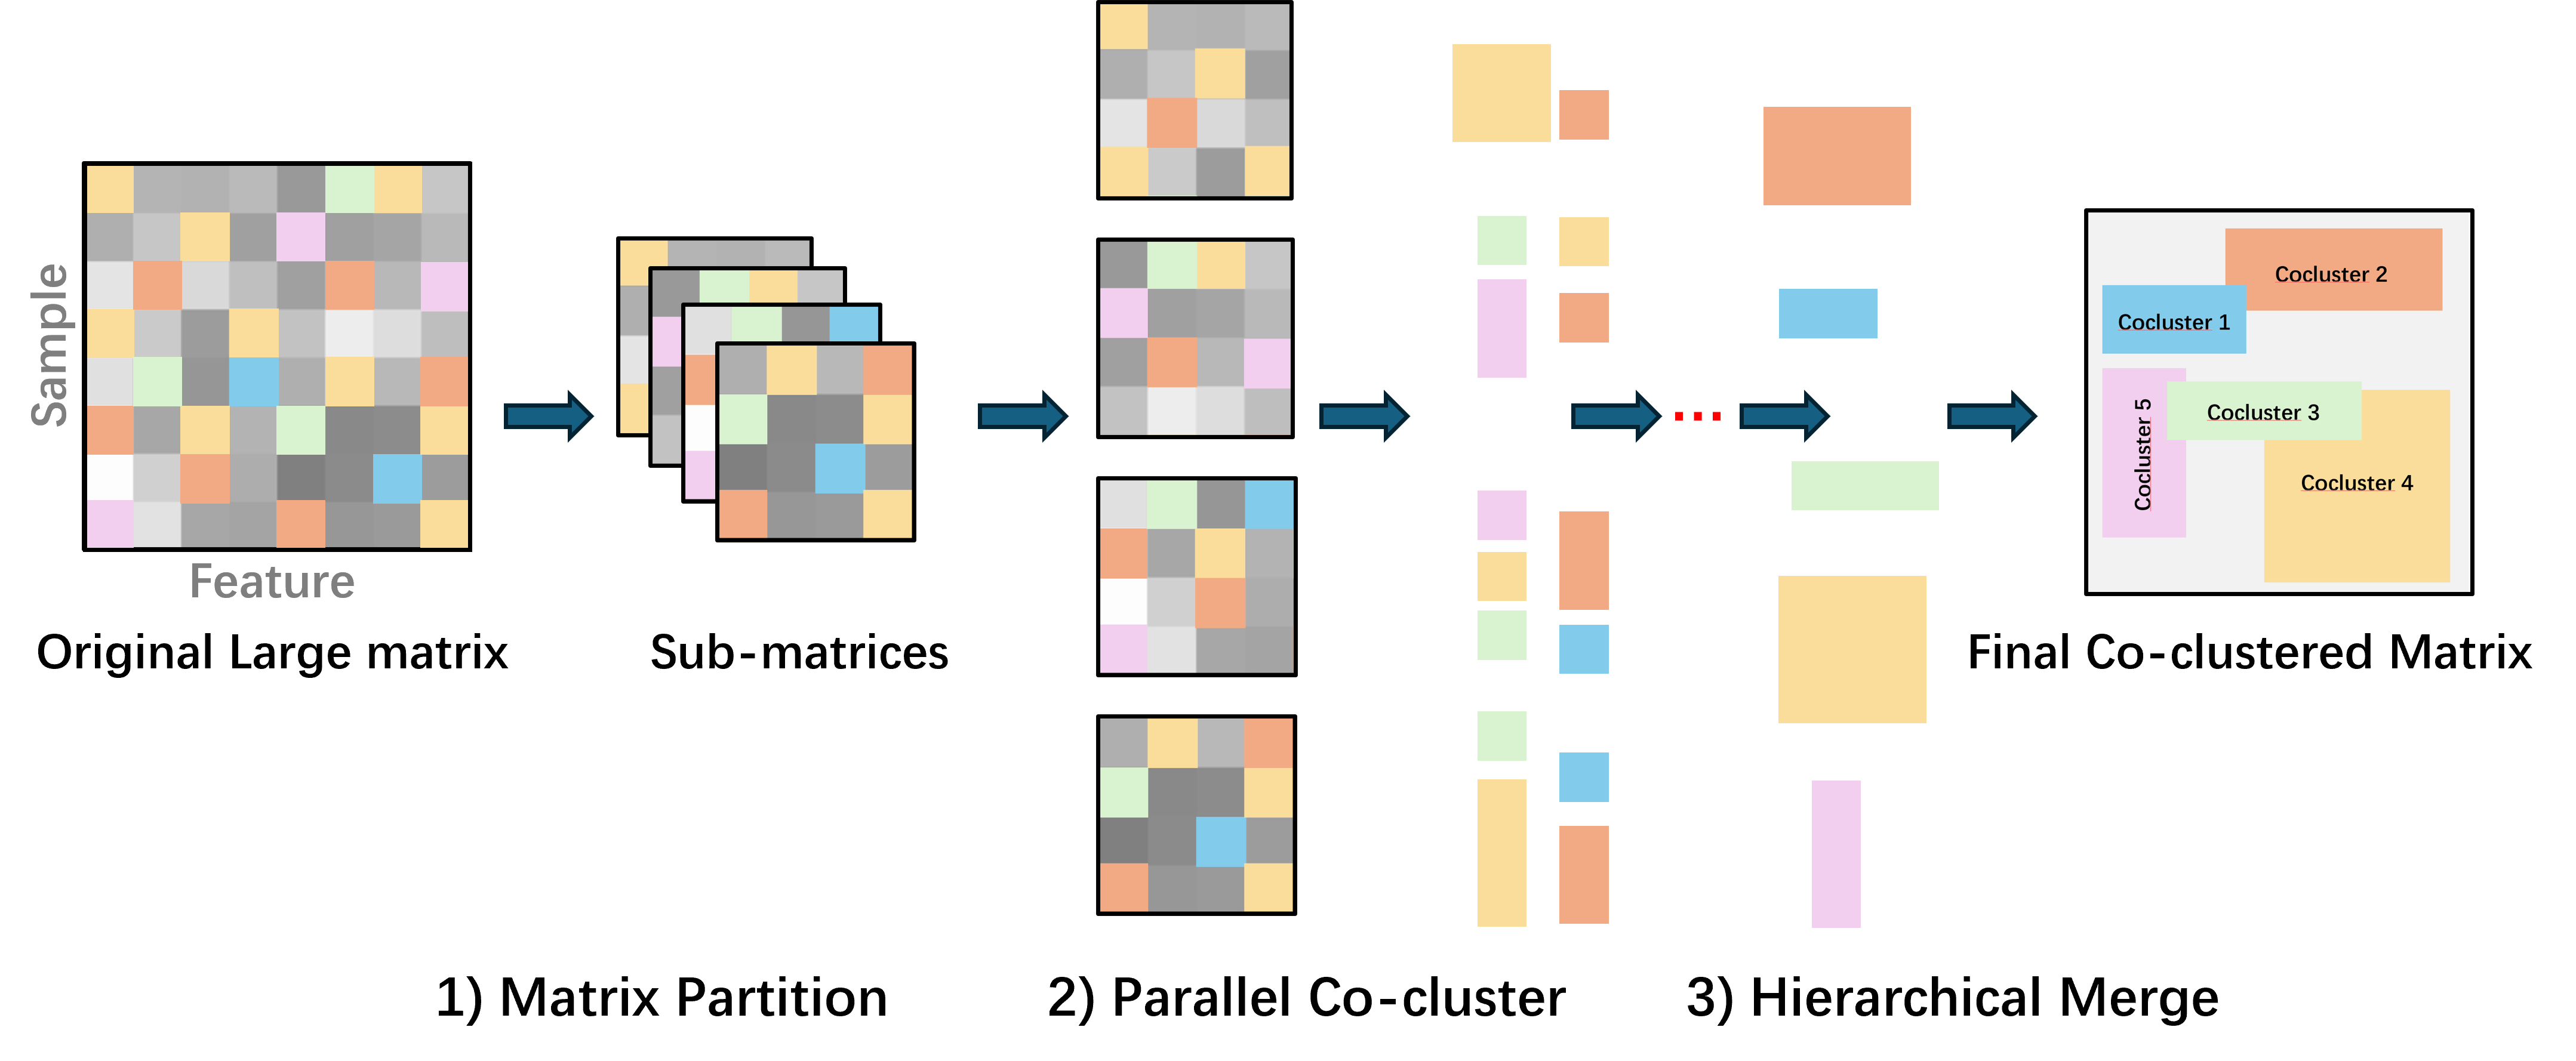
\includegraphics[width=0.8\linewidth]{workflow.png}
  \caption{Workflow of our proposed scalable co-clustering method for large matrices.}
  \label{fig:workflow}
\end{figure*}

This paper presents a novel and scalable co-clustering method specifically designed for large matrices, as shown in \Cref{fig:workflow}. This method applies a probabilistic model-based optimal partitioning algorithm, which not only predicts the ideal number and sequence of partitions for maximizing computational efficiency but also ensures the effectiveness of the co-clustering process.

Our method involves partitioning large matrices into smaller, manageable submatrices. This strategic partitioning is meticulously guided by a probabilistic model, ensuring that the integrity of co-clusters is maintained even as the matrix is divided. After partitioning, each submatrix is handled by a separate computational unit. This approach significantly shortens the processing time and reduces memory consumption for each unit. The probabilistic model serves as a guide, addressing one of the biggest challenges of the partitioning framework: the potential risk of missing small co-clusters. By estimating the likelihood of identifying all relevant co-clusters, the model ensures comprehensive data coverage and robust clustering results, even for smaller, more intricate patterns within the data.

Following the partitioning, each submatrix undergoes a co-clustering process, leveraging the strengths of advanced co-clustering methods. Our approach is modular, allowing any sophisticated co-clustering technique, whether existing or developed in the future, to be applied to each submatrix. This flexibility ensures that the method can be tailored to the unique characteristics of each submatrix, optimizing clustering results. A crucial theorem guarantees the success probability of our framework, provided that the chosen atom co-clustering method is effective in identifying all co-clusters above a certain size with a high probability. This modular design not only enhances the adaptability and robustness of our method but also ensures a comprehensive and accurate co-clustering outcome.

Furthermore, our method integrates a novel hierarchical merging strategy that combines the co-clustering results from all submatrices. This integration provides more fine-grained insights into each submatrix and enhances the overall accuracy and reliability of the co-clustering results. The hierarchical merging process iteratively combines co-clusters from the submatrices, ensuring that the final result is comprehensive and consistent across the entire dataset. Unlike other methods such as NMTF or alternating row and column optimization, our approach guarantees that the iteration number is bounded by a function of the data size, leading to an expected time frame for achieving the ideal result\cite{wang2011FastNonnegativeMatrix}. This multi-step process not only improves scalability but also ensures that the final co-clustering results are robust and reliable, even for very large datasets. Our method, validated and optimized through a comprehensive process, demonstrates unprecedented efficiency in handling large-scale datasets.
More details about the partitioning and co-clustering processes are shown in \Cref{alg:method}.

\begin{algorithm}[!t]
  \caption{Optimal Matrix Partition and Hierarchical Co-cluster Merging Method}\label{alg:method}
  \begin{algorithmic}[1]
    \REQUIRE{Data matrix $\mathbf{A} \in \mathbb{R}^{M \times N}$, Co-cluster set $C = \{C_k\}_{k=1}^K$, Block sizes $\{\phi_i\}_{i=1}^m$, $\{\psi_j\}_{j=1}^n$, Thresholds $T_m$, $T_n$, Sampling times $T_p$, Probability threshold $P_\text{thresh}$;}
    \ENSURE{Co-clustered result $\mathcal{C}$;}
    \STATE Initialize block set $B = \{B_{(i,j)}\}_{i=1}^m,_{j=1}^n$ based on $\phi_i$ and $\psi_j$
    \STATE Calculate $s^{(k)}$ and $t^{(k)}$ for each co-cluster $C_k$
    \FOR{$k=1$ to $K$}
    \STATE Calculate $P(\omega_k)$ for co-cluster $C_k$
    \IF{$P(\omega_k) < P_\text{thresh}$}
    \STATE Partition matrix $A$ into blocks $B$ and perform co-clustering
    \STATE Aggregate co-clustered results from each block
    \ENDIF
    \ENDFOR
    \RETURN Aggregated co-clustered result $\mathcal{C}$
  \end{algorithmic}
\end{algorithm}

In the following sections, we begin by introducing the large matrix partitioning algorithm, which forms the cornerstone of our scalable co-clustering method. Following this, we describe the atom-co-clustering algorithm, designed for compatibility with our framework and suitable for application to each submatrix. For completeness, we also present a graph-based spectral co-clustering algorithm that can be seamlessly integrated into our framework for submatrix processing. Afterward, we explain the hierarchical merging algorithm, which efficiently combines the co-clustering results from all submatrices. Finally, we detail the MPI implementation of our method, demonstrating its feasibility and effectiveness in multi-node scenarios.

\subsection{Large Matrix Partitioning}

The primary challenge in co-clustering large matrices is the risk of losing meaningful co-cluster relationships when the matrix is partitioned into smaller submatrices. To address this, we introduce an optimal partitioning algorithm underpinned by a probabilistic model. This model is meticulously designed to navigate the complexities of partitioning, ensuring that the integrity of co-clusters is maintained even as the matrix is divided. The objective of this algorithm is twofold: to determine the optimal partitioning strategy that minimizes the risk of fragmenting significant co-clusters and to define the appropriate number of repartitioning iterations needed to achieve a desired success rate of co-cluster identification.

\subsubsection{Partitioning and Repartitioning Strategy based on the Probabilistic Model}

Our probabilistic model serves as the cornerstone of the partitioning algorithm. It assures all co-clusters above a demarcated size threshold are identified with a high probability, guiding the partitioning process to minimize the risk of losing critical co-cluster relationships. The model is based on the following assumptions:

In the scenario where the matrix $A$ is partitioned into $m \times n$ blocks, each block has size $\phi_i \times \psi_j$, that is, $M=\sum_{i=1}^m \phi_i$ and $N=\sum_{j=1}^n \psi_j$, the joint probability of $M_{(i,j)}^{(k)}$ and $N_{(i,j)}^{(k)}$ is given by \Cref{thm:joint_probability}:
\begin{align*}
  P(M_{(i,j)}^{(k)} & < T_m, N_{(i,j)}^{(k)} < T_n)                                                                           \\
                    & = \sum_{\alpha=1}^{T_m-1} \sum_{\beta=1}^{T_n-1} P(M_{(i,j)}^{(k)} = \alpha) P(N_{(i,j)}^{(k)} = \beta) \\
                    & \le \exp[-2 (s_i^{(k)})^2 \phi_i + -2 (t_j^{(k)})^2 \psi_j]
\end{align*}
where $s_i^{(k)}$ and $t_j^{(k)}$ are the minimum row and column sizes of co-cluster $C_k$ in block $B_{(i,j)}$, the size of the co-cluster $C_k$ is $M^{(k)} \times N^{(k)}$, and $M^{(k)}$ and $N^{(k)}$ are the row and column sizes of co-cluster $C_k$, respectively.

Thus, $P$, the probability of identifying all co-clusters is given by \Cref{thm:probability_co_cluster_detection}:

\begin{align}
  P \ge 1 - \exp \left\{ -2 T_p [\phi m (s^{(k)})^2 + \psi n (t^{(k)})^2] \right\} \label{eq:prob_of_identifying_all_co_clusters}
\end{align}
where $P(\omega_k)$ is the probability of the failure of identifying co-cluster $C_k$, $T_p$ is the number of sampling times, $\phi$ and $\psi$ are the row and column block sizes, and $s^{(k)}$ and $t^{(k)}$ are the minimum row and column sizes of co-cluster $C_k$.

\Cref{eq:prob_of_identifying_all_co_clusters} is central to our algorithm for partitioning large matrices for co-clustering, providing a probabilistic model that informs and optimizes our partitioning strategy to preserve co-cluster integrity. It mathematically quantifies the likelihood of identifying all relevant co-clusters within partitioned blocks, guiding us to mitigate risks associated with partitioning that might fragment vital co-cluster relationships.

Based on \Cref{eq:prob_of_identifying_all_co_clusters}, we can establish a constraint between the partitioning time $T_p$ and the partition solution $Par(\{\phi_i\}_{i=1}^m, \{\psi_j\}_{j=1}^n)$, ensuring that the partitioning strategy adheres to a predetermined tolerance success rate, thereby minimizing the risk of co-cluster fragmentation.

\subsubsection{Optimization and Computational Efficiency}

Optimizing the partitioning process for computational efficiency is critical in both academic and industrial applications, where running time is often the primary bottleneck. Our optimization strategy leverages the probabilistic model and constraints derived in \Cref{eq:prob_of_identifying_all_co_clusters} to balance computational resource allocation and adherence to theoretical success thresholds.

Our approach systematically evaluates various partitioning configurations to minimize running time without compromising the integrity and success rate of co-cluster identification. The key condition for optimizing the partitioning algorithm, while maintaining a predetermined success rate \( P \) for co-cluster identification, is given by:

\begin{align*}
  T_p = \text{argmin}_{T_p} \{
  1 & - \exp \{ -2 T_p [\phi m (s^{(k)})^2         \\
    & + n (t^{(k)})^2] \} \ge P_{\text{thresh}} \}
\end{align*}

This condition delineates the parameters within which the partitioning strategy can be optimized for speed without sacrificing the algorithm's ability to accurately identify co-clusters. By adhering to this theorem, we ensure that our optimization efforts preserve the integrity and effectiveness of co-cluster discovery, making the partitioning algorithm fast, efficient, and robust across various datasets and co-clustering challenges.

\subsubsection{Noisy Case Analysis}

In the presence of noise, the partitioning algorithm must be adapted to account for the additional complexity introduced by noisy data. The probabilistic model, which forms the foundation of our partitioning strategy, can be extended to accommodate noisy data by incorporating noise parameters into the co-cluster score function. This extension allows the model to evaluate the impact of noise on co-cluster identification and adjust the partitioning strategy accordingly. More details can be found in \Cref{subsubsec:noisy_case}.
\subsection{Co-clustering on Small Submatrices}

\subsubsection{Atom-co-clustering Algorithm}

Our framework, which encompasses both partitioning and ensembling, offers remarkable flexibility, allowing it to

be compatible with a wide range of atom-co-clustering methods. For the sake of making this paper comprehensive and self-contained, we provide an introduction to the atom-co-cluster method herein. The only requirement for an atom-co-clustering method to be compatible with our framework is that it must be able to identify co-clusters under a given criterion with a probability $p$, or more relaxed conditions, has a lower bound estimate of the probability of identifying co-clusters equipped with a validation mechanism.

\subsubsection{Graph-based Spectral Co-clustering Algorithm}

Spectral co-clustering (SCC) stands as one of the most prevalent methods in the realm of co-clustering today \cite{vonluxburg2007TutorialSpectralClustering}, primarily due to its adeptness in unraveling the complexities of high-dimensional data. At its core, this method harnesses the power of spectral clustering principles, focusing on the utilization of a graph's Laplacian matrix eigenvectors for effectively partitioning data into distinct clusters. This approach is exceptionally beneficial for analyzing data that naturally forms a bipartite graph structure, including applications in text-document analysis, social network modeling, and gene expression studies.

\paragraph{Graph Construction in Co-clustering Expanded}

SCC begins with constructing a bipartite graph $G=(U,V,E)$. Here, $U$ and $V$, both as vertex sets, symbolize the sets corresponding to the rows and columns of the data matrix, respectively. The edges $E$ of this graph are assigned weights reflecting the relationships between rows and columns. Consequently, the graph's weighted adjacency matrix $W$ is defined as:

$$ W = \begin{bmatrix} 0 & A \\ A^T & 0 \end{bmatrix}, $$
where $A$ denotes the data matrix, also called the adjacency matrix in the graph context.
Through this representation, the challenge of co-clustering is reformulated into a graph partitioning task, aiming to segregate the graph into distinct clusters based on the interrelations between the data matrix's rows and columns.

\paragraph{Laplacian Matrix}

The graph's Laplacian matrix $L$ is computed as $L=D-W$, with $D$ being the graph's degree matrix—a diagonal matrix whose entries equal the sum of the weights of the edges incident to each node. The Laplacian matrix plays a crucial role in identifying the graph's cluster structure. It does so by facilitating the calculation of eigenvectors associated with its smallest positive eigenvalues, which in turn, guide the partitioning of the graph into clusters.

\paragraph{Graph Partitioning and Singular Value Decomposition}

Theorem 4 in \cite{dhillon2001CoclusteringDocumentsWords} states that the eigenvector corresponding to the second smallest eigenvalue of the following eigenvalue problem gives the generalized partition vectors for the graph:

\begin{equation}
  L \mathbf{v} = \lambda D \mathbf{v}
  \label{eq:eigenvalue_problem}
\end{equation}

And according to Section 4 of \cite{dhillon2001CoclusteringDocumentsWords}, the singular value decomposition of the normalized matrix $A_n = D^{-1/2} A D^{-1/2}$
$$A_n = U \Sigma V^T$$
gives the solution to \Cref{eq:eigenvalue_problem}. To be more specific, the singular vectors corresponding to the second largest singular value of $A_n$ are the eigenvector corresponding to the second smallest eigenvalue of \Cref{eq:eigenvalue_problem}.

The above discussion is under the assumption that the graph has only one connected component. In a more general setting, $\mathbf{u_2}, \mathbf{u_3}, \ldots, \mathbf{u_{l+1}}$ and $\mathbf{v_2}, \mathbf{v_3}, \ldots, \mathbf{v_{l+1}}$ reveal the $k$-modal information of the graph, where $\mathbf{u_k}$ and $\mathbf{v_k}$ are the $k$-th left and right singular vectors of $A_n$, respectively. And for the last step,
$$ Z = \begin{bmatrix} D_1^{-1/2} \hat{U} \\ D_2^{-1/2} \hat{V} \end{bmatrix} $$
is stacked where $\hat{U} = [\mathbf{u_2}; \mathbf{u_3}; \ldots; \mathbf{u_{l+1}}]$ and $\hat{V} = [\mathbf{v_2}; \mathbf{v_3}; \ldots; \mathbf{v_{l+1}}]$. The approximation to the graph partitioning optimization problem is then solved by applying a $k$-means algorithm to the rows of $Z$. More details can be found in \cite{dhillon2001CoclusteringDocumentsWords}.

\subsubsection{Hierarchical Co-cluster Merging}

Hierarchical co-cluster merging is a novel approach that combines the results of co-clustering on submatrices to produce a final co-clustered result. The merging method is designed to enhance the accuracy and robustness of the co-clustering outcome by leveraging the design of the partitioning algorithm. The hierarchical merging process iteratively combines the co-clusters from each submatrix, ensuring that the final co-clustered result is comprehensive and consistent across all submatrices. This iterative merging process is crucial for addressing issues of heterogeneity and model uncertainty, ensuring that the final co-clustering results are reliable and robust. The hierarchical merging algorithm is detailed in \Cref{alg:hierarchical_merging}.

\begin{itemize}
  \item \textbf{Merging Small Co-clusters:} Each pair of identified small co-clusters is considered for merging. The merging decision is based on a scoring system as shown in Definition~\ref{def:co_cluster}, where the score is derived from performing SVD on a matrix and calculating the ratio of the second largest eigenvalue to the largest eigenvalue. This score is regularized by dividing it with the Frobenius norm of the matrix. If the score of the merged co-cluster is not higher than that of any smaller co-cluster, the merging is considered successful, indicating the formation of a larger co-cluster.
  \item \textbf{Efficiency through Overlap Check:} To accelerate the process, the algorithm checks if the co-clusters overlap in the larger matrix. Merging is only attempted for co-clusters that share common rows or columns. This strategy not only speeds up the merging process but also reduces the computational complexity.
\end{itemize}

\begin{algorithm}[!t]
  \caption{Hierarchical Co-cluster Merging Algorithm}\label{alg:hierarchical_merging}
  \begin{algorithmic}[1]
    \REQUIRE{Set of co-clusters $\mathcal{C}$ from submatrices, data matrix $A \in \mathbb{R}^{M \times N}$, threshold for score improvement $\tau$;}
    \ENSURE{Final co-clustered result $\mathcal{C}_{\text{final}}$;}

    \STATE Initialize $\mathcal{C}_{\text{final}} = \mathcal{C}$
    \STATE Calculate initial scores for all co-clusters in $\mathcal{C}$

    \WHILE{true}
    \STATE $merged = \text{False}$
    \FOR{each pair of co-clusters $(C_i, C_j)$ in $\mathcal{C}_{\text{final}}$}
    \IF{$C_i$ and $C_j$ have common rows or columns}
    \STATE Merge $C_i$ and $C_j$ to form $C_{ij}$
    \STATE Perform SVD on $C_{ij}$ and calculate the score
    \IF{score of $C_{ij}$ $\leq$ score of $C_i$ and score of $C_{ij}$ $\leq$ score of $C_j$}
    \STATE Replace $C_i$ and $C_j$ with $C_{ij}$ in $\mathcal{C}_{\text{final}}$
    \STATE Update the scores for the affected co-clusters
    \STATE $merged = \text{True}$
    \ENDIF
    \ENDIF
    \ENDFOR
    \IF{not $merged$}
    \STATE Break
    \ENDIF
    \ENDWHILE

    \RETURN $\mathcal{C}_{\text{final}}$
  \end{algorithmic}
\end{algorithm}

In this algorithm, steps 1 and 2 initialize the final co-cluster set and calculate initial scores for all co-clusters. The while loop iteratively attempts to merge co-clusters until no further merging is possible. Within the loop, the algorithm checks for overlaps and calculates scores for potential merges. If the score of a merged co-cluster does not exceed the scores of its components, the merge is accepted, and the final co-cluster set is updated accordingly. This approach ensures a scalable and efficient merging process while maintaining the integrity and robustness of the co-clustering results.

\subsection{MPI Implementation}

Our proposed scalable co-clustering method is implemented using the Message Passing Interface (MPI) to enable distributed computing across multiple nodes. This implementation allows for effective distribution of the computational load, facilitating parallel processing of submatrices and enhancing the scalability of our method. The main computation node is responsible for computing thresholds based on the size of the matrix, without requiring specialized performance beyond that of other nodes. This design ensures that our approach is practical and scalable for large-scale applications, without the need for a supercomputer or high-performance central processing unit.
More details about the MPI implementation are shown in \Cref{alg:mpi_method}.

In conclusion, our proposed scalable co-clustering method effectively addresses the challenges associated with large-scale data analysis. By leveraging a probabilistic model for optimal partitioning and a hierarchical merging strategy, we ensure that our method is both efficient and robust. The detailed algorithmic framework and theoretical underpinnings provide a solid foundation for further research and development in this field.

\begin{algorithm}[!t]
  \caption{MPI-based Optimal Matrix Partition and Hierarchical Co-cluster Merging Method}\label{alg:mpi_method}
  \begin{algorithmic}[1]
    \REQUIRE{Data matrix $\mathbf{A} \in \mathbb{R}^{M \times N}$, Co-cluster set $C = \{C_k\}_{k=1}^K$, Block sizes $\{\phi_i\}_{i=1}^m$, $\{\psi_j\}_{j=1}^n$, Thresholds $T_m$, $T_n$, Sampling times $T_p$, Probability threshold $P_\text{thresh}$, Number of processors $P$;}
    \ENSURE{Co-clustered result $\mathcal{C}$;}
    \STATE Initialize MPI environment
    \STATE Determine rank and size using \texttt{MPI\_Comm\_rank} and \texttt{MPI\_Comm\_size}
    \IF{rank == 0}
    \STATE Initialize block set $B = \{B_{(i,j)}\}_{i=1}^m,_{j=1}^n$ based on $\phi_i$ and $\psi_j$
    \STATE Calculate $s^{(k)}$ and $t^{(k)}$ for each co-cluster $C_k$
    \FOR{$k=1$ to $K$}
    \STATE Calculate $P(\omega_k)$ for co-cluster $C_k$
    \IF{$P(\omega_k) < P_{thresh}$}
    \STATE Partition matrix $\mathbf{A}$ into blocks $B$ and distribute to processors
    \FOR{each processor $p$}
    \STATE Send corresponding block $B_p$ to processor $p$
    \ENDFOR
    \ENDIF
    \ENDFOR
    \ENDIF
    \STATE Each processor $p$ receives its block $B_p$ and performs co-clustering
    \STATE Each processor sends its co-clustered result $C_p$ back to the root processor
    \IF{rank == 0}
    \STATE $\mathcal{C}$ $\gets$ Aggregate co-clustered results from all blocks
    \RETURN Aggregated co-clustered result $\mathcal{C}$
    \ENDIF
    \STATE Finalize MPI environment
  \end{algorithmic}
\end{algorithm}

\section{Complexity and Probability Analysis}

\label{sec:analysis}

\subsection{Complexity Analysis}
\label{subsec:complexity}
In this section, we analyze the complexity of our proposed scalable co-clustering method. We begin by comparing the space and time complexity with traditional co-clustering methods. Then, we discuss the communication cost in a distributed computing environment.

\subsection{Space Complexity Comparison}

The memory requirement for traditional co-clustering methods, such as Non-negative Matrix Tri-Factorization (NMTF), involves the storage of the input data matrix $X$ of size $O(IT)$, output factor matrices $Z$, $S$, and $W$ of size $O(IJ_1 + TJ_2 + J_1J_2)$, and several temporary matrices of size $O(TJ_1 + IJ_2 + J_1^2 + J_2^2)$. The total space complexity for NMTF is $O(IT + (I + T)(J_1 + J_2) + J_1J_2 + J_1^2 + J_2^2)$.

However, due to the sequential computation of NMTF, all matrices need to be stored on a single computing node, leading to significant memory constraints. In contrast, our method distributes the storage across multiple nodes. For each node, the memory requirement includes blocks of input data matrices $X_{\text{row}}$ and $X_{\text{col}}$ of size $O(\frac{2IT}{p})$, blocks of factor matrices $Z_{\text{row}}$ and $W_{\text{row}}$ of size $O(\frac{IJ_1 + TJ_2}{p})$, and the factor matrix $S$ along with auxiliary matrices of size $O(J_1J_2 + IJ_1 + J_1^2 + TJ_2 + J_2^2)$. The temporary matrices require $O(\frac{TJ_1 + IJ_2}{p} + J_1^2 + J_2^2 + J_1J_2)$. The total space complexity for our method is $O(\frac{IT + (I + T)(J_1 + J_2)}{p} + IJ_1 + TJ_2 + J_1J_2 + J_1^2 + J_2^2)$.

Compared to NMTF, our method alleviates the problem of excessive storage by distributing data matrices, making it more applicable for real-world datasets.

\subsection{Time Complexity Comparison}

The computational bottleneck of NMTF lies in the matrix multiplications within the multiplicative update formulas. The complexity for these operations is $O(IT(J_1 + J_2) + (I + T)(J_1^2 + J_2^2 + J_1J_2) + J_1^2J_2 + J_1J_2^2)$.

Our method, designed to operate in parallel, also focuses on reducing this computational load. The solving procedure of a linear system in each iteration, the most time-consuming operation, has a complexity of $O(J_1^3)$ or $O(J_2^3)$. Thus, the total time complexity for our method is $O(\frac{IT(J_1 + J_2) + (I + T)(J_1^2 + J_2^2 + J_1J_2) + J_1^2J_2 + J_1J_2^2}{p})$.

This parallel approach reduces the computational burden by distributing tasks across multiple nodes, making our method more efficient than traditional NMTF.

\subsection{Communication Cost Analysis}

To analyze the communication cost, we apply the $\alpha$-$\beta$-$\gamma$ model of distributed-memory parallel computation. In this model, the cost of passing a message of $n$ words is modeled as $\alpha + n\beta$, where $\alpha$ is the latency cost and $\beta$ is the per-word bandwidth cost. Each process performs computation with a per-flop computation cost $\gamma$.

% The major communication cost of our method is associated with collective operations such as \textit{Reduce_Scatter} and \textit{Allreduce}. The communication costs for these operations are $O(\alpha \cdot \log p + (\beta + \gamma) \cdot \frac{p-1}{p} n)$ and $O(2\alpha \cdot \log p + (2\beta + \gamma) \cdot \frac{p-1}{p} n)$, respectively.

For lines 10, 16, and 21 in our algorithm, the communication costs are $O(\alpha \cdot \log p + (\beta + \gamma) \cdot \frac{p-1}{p} IJ_1)$, $O(\alpha \cdot \log p + (\beta + \gamma) \cdot \frac{p-1}{p} TJ_2)$, and $O(\alpha \cdot \log p + (\beta + \gamma) \cdot \frac{p-1}{p} J_1T)$, respectively. Similarly, the communication costs for lines 12, 18, 23, 25, and 27 are $O(2\alpha \cdot \log p + (2\beta + \gamma) \cdot \frac{p-1}{p} J_2^2)$, $O(2\alpha \cdot \log p + (2\beta + \gamma) \cdot \frac{p-1}{p} J_1J_2)$, and $O(2\alpha \cdot \log p + (2\beta + \gamma) \cdot \frac{p-1}{p} J_1^2)$, respectively.

Therefore, the major communication cost of our method is $O(2\alpha \cdot \log p + (\beta + \gamma)((I + T)J_1 + TJ_2) + (2\beta + \gamma)(J_1^2 + J_2^2 + J_1J_2))$, which shows that our method effectively balances computation and communication costs in a distributed environment.

\subsection{Probability Analysis}

\subsubsection{Notations}
\label{subsec:probability}
\begin{itemize}
  \item $\mathbf{A} \in \mathbb{R}^{M \times N}$ is a matrix with $K$ co-clusters (co-cluster set $\mathcal{C} = \{\mathbf{C}_k\}_{k=1}^K$);
  \item $\mathbf{A}$ is partitioned into $m \times n$ blocks, each block has size $\phi_i \times \psi_j$, that is, $M=\sum_{i=1}^m \phi_i$ and $N=\sum_{j=1}^n \psi_j$;
  \item thus block set $\mathbf{B} = \{\mathbf{B}_{(i,j)}\}_{i=1}^m,_{j=1}^n$;
  \item the size of co-cluster $\mathbf{C}_k \in \mathbb{R}^{M^{(k)} \times N^{(k)}}$ that falls into block $\mathbf{B}_{(i,j)}$ is $M_{(i,j)}^{(k)} \times N_{(i,j)}^{(k)}$;
  \item $T_m$ is the minimum number of rows, $T_n$ is the minimum number of columns.
\end{itemize}

\subsubsection{Probability}

\begin{lemma}[Joint Probability of Co-cluster Size]
  \label{thm:joint_probability}
  Let $C_k$ be a co-cluster and $B_{(i,j)}$ be a block in the partitioned matrix. The probability that the size of the co-cluster $C_k$ within block $B_{(i,j)}$ is less than $T_m$ rows and $T_n$ columns is given by:
  \begin{align*}
    P(M_{(i,j)}^{(k)} < T_m, N_{(i,j)}^{(k)} < T_n) & \le \exp[-2 (s_i^{(k)})^2 \phi_i -2 (t_j^{(k)})^2 \psi_j]
  \end{align*}
  where $s_i^{(k)} = \cfrac{M^{(k)}}{M}-\cfrac{T_m-1}{\phi_i}$ and $t_j^{(k)} = \cfrac{N^{(k)}}{N}-\cfrac{T_n-1}{\psi_j}$.
\end{lemma}

This lemma provides a mathematical foundation for estimating the likelihood of a co-cluster's size being below a specified threshold within any given block. It helps us understand how partitioning impacts the detection of small co-clusters.

\begin{theorem}
  \label{thm:probability_co_cluster_detection}
  If the matrix $\mathbf{A}$ is partitioned into $m \times n$ blocks, each with sizes $\phi_i \times \psi_j$, and the probability of failing to detect co-cluster $\mathbf{C}_k$ in any block is $P(\omega_k)$, then
  \begin{align*}
    P(\omega_k) & \le \exp \left\{ -2 [\phi m (s^{(k)})^2 + \psi n (t^{(k)})^2] \right\}
  \end{align*}
  Given $T_p$ times of random sampling, the probability of detecting the co-cluster $C_k$ is
  \begin{align*}
    P & = 1 - P(\omega_k)^{T_p}                                                        \\
      & \ge 1 - \exp \left\{ -2 T_p [\phi m (s^{(k)})^2 + \psi n (t^{(k)})^2] \right\}
  \end{align*}
  This can be used to set $m, n, \phi, \psi, T_m, T_n$, and $T_p$ to ensure the probability of detecting the co-cluster is larger than a given threshold.
\end{theorem}

This theorem allows us to determine the optimal partitioning parameters to maximize the probability of detecting co-clusters. It provides a theoretical guarantee for the success of our partitioning strategy by specifying conditions under which co-cluster detection is highly probable.

\subsubsection{Noisy Case}
\label{subsubsec:noisy_case}

\begin{assumption}
  Assume each noise $n_{ij}$ follows a normal distribution $N(0, \sigma^2)$, independently and identically distributed (i.i.d.) for all $i$ and $j$. Suppose there exists $\lambda > 0$, such that
  $$\lambda \le \max(||\mathbf{B}||_1, ||\mathbf{B}^\top||_1)/\sigma^2.$$
\end{assumption}

\begin{definition}
  The score of a submatrix $\mathbf{A}_{I,J}$ is defined as
  \begin{align}
    S(I,J)       & = \min(S_{row}(I,J), S_{col}(I,J))                                                                                          \\
    S_{row}(I,J) & = \min_{i_1, i_2 \in I} \left(1- \frac{1}{|I|-1} \sum_{i_2 \in I, i_2 \neq i_1} \langle x_{i_1,J}, x_{i_2,J}\rangle \right) \\
    S_{col}(I,J) & = \min_{j_1, j_2 \in J} \left(1- \frac{1}{|J|-1} \sum_{j_2 \in J, j_2 \neq j_1} \langle x_{I,j_1}, x_{I,j_2}\rangle \right)
  \end{align}
  where $x_{i,J}$ is the $i$-th row of $A_{I,J}$ and the inner product $\langle x, y \rangle$ is defined as
  $$\langle x, y \rangle = \exp(-\frac{||x - y||_1^2}{2\alpha||x||_1||y||_1})$$
\end{definition}

The score function $S(I,J)$ measures the similarity within a submatrix, considering both row and column relationships. This metric is crucial for evaluating the quality of co-clustering under noisy conditions.

\begin{theorem}
  \label{thm:expected_score}
  Given the hidden co-cluster matrix $A$ and noise matrix $\mathbf{E}$, the observed matrix is $\mathbf{B} = \mathbf{A} + \mathbf{E}$. The expected value and variance of $S_{row}(I,J)$ are:
  \begin{align*}
    \mathbb{E}(S_{row}(I,J)) & \ge |J||I| \left(1 - \exp(-\frac{2}{\alpha \max(||\mathbf{B}||_1, ||\mathbf{B}^\top||_1)}) \right) \\
    \sigma^2(S_{row}(I,J))   & \le |I||J| \sigma^2 \exp(-\frac{2}{\alpha \max(||\mathbf{B}||_1, ||\mathbf{B}^\top||_1)})
  \end{align*}
  Similarly, for $S_{col}(I,J)$:
  \begin{align*}
    \mathbb{E}(S_{col}(I,J)) & \ge |J||I| \left(1 - \exp(-\frac{2}{\alpha \max(||\mathbf{B}||_1, ||\mathbf{B}^\top||_1)}) \right) \\
    \sigma^2(S_{col}(I,J))   & \le |I||J| \sigma^2 \exp(-\frac{2}{\alpha \max(||\mathbf{B}||_1, ||\mathbf{B}^\top||_1)})
  \end{align*}
\end{theorem}

This theorem establishes the expected behavior of the score function $S(I,J)$ under noise, providing insights into how noise impacts the similarity measures used in our co-clustering method.

\begin{theorem}
  \label{thm:chernoff_bound}
  According to the Chernoff bound, the probability that $S(I,J)$ is close to its expected value is:
  \begin{align*}
    P(S(I,J) \le \mathbb{E}(S(I,J)) - \epsilon)
     & \ge \exp(-\frac{\epsilon^2}{2|I||J| \sigma^2 \exp(-\frac{2}{\alpha \lambda})})
  \end{align*}
  Setting $\epsilon = \sqrt{2|I||J| \sigma^2 \exp(-\frac{2}{\alpha \lambda}) \log(1/\delta)}$, we have:
  \begin{align*}
    P(S(I,J) \ge \mathbb{E}(S(I,J)) - \epsilon) & \ge \delta
  \end{align*}
  Combining this with the probability control of $T_p$, we can select parameters to ensure the probability of detecting the co-cluster is larger than a given threshold.
\end{theorem}

This theorem uses the Chernoff bound to quantify the likelihood that the score function $S(I,J)$ will remain close to its expected value, even in the presence of noise. By appropriately selecting parameters, we can ensure high confidence in detecting co-clusters despite noisy data.

\section{Experiment Evaluation}
\label{sec:experiment}


\begin{table*}[htbp]
  \centering
  \caption{Comparison of Running Times (in seconds) for Various Co-clustering Methods on Selected Datasets.}
  \label{tab:running-time}
  \begin{tabular}{@{} l cccccccc @{}}
    \toprule
    Dataset     & SCC \cite{dhillon2001CoclusteringDocumentsWords}
                & NMTF \cite{long2005CoclusteringBlockValue}
                & ONMTF \cite{ding2006OrthogonalNonnegativeMatrix}
                & WC-NMTF \cite{salah2018WordCooccurrenceRegularized}
                & FNMTF \cite{kim2011FastNonnegativeMatrix}
                & PNMTF \cite{chen2023ParallelNonNegativeMatrix}      & \textbf{MPHM-SCC} & \textbf{MPHM-PNMTF}                                                \\
    \midrule
    Amazon 1000 & 64545.2                                             & 298.7             & 498.4               & 198.8  & 275.1  & 303.7   & 112.5  & 242.8   \\
    CLASSIC4    & *                                                   & 75,530            & 68,793              & 27,114 & 189,47 & 17,810  & 22,894 & 3,028   \\
    RCV1-Large  & *                                                   & *                 & *                   & *      & *      & 277,092 & *      & 208,048 \\
    % ... more rows here
    \bottomrule
  \end{tabular}
  \begin{tablenotes}
    \small
    \item Notes: * indicates that the method cannot process the dataset because the dataset size exceeds the processing limit.
  \end{tablenotes}
\end{table*}

\begin{table*}[htbp]
  \centering
  \caption{NMIs and ARIs Scores for Various Co-clustering Methods on Selected Datasets.}
  \label{tab:evaluation-metrics}
  \begin{tabular}{@{} l c cccc @{}}
    \toprule
    \multirow{2}{*}{Dataset}     & \multirow{2}{*}{Metric} & \multicolumn{4}{c}{Compared Methods}                                                                                                        \\
    \cmidrule{3-6}
                                 &                         & SCC \cite{dhillon2001CoclusteringDocumentsWords} & PNMTF \cite{chen2023ParallelNonNegativeMatrix} & \textbf{MPHM-SCC} & \textbf{MPHM-PNMTF} \\
    \midrule
    \multirow{2}{*}{Amazon 1000} & NMI                     & 0.9223                                           & 0.6894                                         & 0.8650            & 0.6609              \\
                                 & ARI                     & 0.7713                                           & 0.6188                                         & 0.7763            & 0.6057              \\
    \multirow{2}{*}{CLASSIC4}    & NMI                     & *                                                & 0.5944                                         & 0.7676            & 0.6073              \\
                                 & ARI                     & *                                                & 0.4523                                         & 0.5845            & 0.4469              \\
    \multirow{2}{*}{RCV1-Large}  & NMI                     & *                                                & 0.6519                                         & 0.8349            & 0.6348              \\
                                 & ARI                     & *                                                & 0.5383                                         & 0.7576            & 0.5298              \\
    % ... more rows here
    \bottomrule
  \end{tabular}
  \begin{tablenotes}
    \small
    \item Notes: * indicates that the method cannot process the dataset because the dataset size exceeds the processing limit.
  \end{tablenotes}
\end{table*}


This section presents the empirical evaluation of the proposed co-cluster method. The experiments aim to assess the method's efficiency, scalability, and accuracy when applied to large data matrices. More experiments on varying the computation units numbers and partition settings show the ability of parallel acceleration and verify the optimal setting proposed respectivley.

\subsection{Experiment Setup}

\begin{table}[h]
  \centering
  \caption{Statistics of Datasets}
  \label{tab:dataset-statistics}
  % \setlength{\tabcolsep}{9pt} % Adjust column separation
  \begin{tabular}{lccc@{}c@{}c@{}c}
    \hline
    \textbf{Dataset} & \textbf{\#Docs} & \textbf{\#Words} & \textbf{\#Clus} & \textbf{Sparsity (\%)} & \textbf{Balance (\%)} \\
    \hline
    CLASSIC4         & 6,461           & 4,667            & 4               & 0.95                   & 40.2                  \\
    Amazon           & 123,321         & 23,379           & 24              & 0.20                   & 75.4                  \\
    RCV1-Large       & 685,071         & 90,210           & 4               & 0.08                   & 18.3                  \\
    \hline
  \end{tabular}
\end{table}

\textbf{Datasets.}
The experiments were conducted using three distinct datasets (see Table \ref{tab:dataset-statistics}) to demonstrate the versatility and robustness of our method:

\begin{itemize}
  \item Amazon 1000: Comprising 1000 Amazon reviews; each represented as a 1000-dimensional vector, this dataset is designed to mimic customer behavior analysis.
  \item CLASSIC4: Containing 18000 documents from 20 newsgroups; each document is represented as a 1000-dimensional vector, this dataset is suitable for text analysis and topic discovery.
  \item RCV1-Large: A larger dataset used to test the scalability of our method, it includes a vast array of document vectors for high-dimensional data analysis.
\end{itemize}

\textbf{Implementation details.}
All experiments were performed on a computing cluster with the following specifications: Intel Xeon E5-2670 v3 @ 2.30GHz processors, 128GB RAM, and Ubuntu 20.04 LTS operating system. The algorithms were implemented in Rust and compiled with the latest stable version of the Rust compiler.

\textbf{Compared Methods.}
The experiments followed the procedure outlined in Algorithm \ref{alg:method}. The proposed method was compared with the following state-of-the-art co-clustering methods:

\begin{itemize}
  \item Spectral Co-Clustering (SCC) \cite{dhillon2001CoclusteringDocumentsWords}
  \item Parallel Non-negative Matrix Tri-Factorization (PNMTF)\cite{chen2023ParallelNonNegativeMatrix}
  \item Deep Co-Clustering (DeepCC)\cite{dongkuanxu2019DeepCoClustering}
\end{itemize}

Notably, 1) PNMTF is one of the most efficient co-clustering algorithms in the state-of-art. 2) All our experiments show that DeepCC cannot process all selected datasets due to the dataset size exceeds DeepCC processing limit.

\textbf{Our Methods.} Our proposed scalable co-cluster method is applied along with the SCC and PNMTF to demonstrate the enhanced performance and capability of handling large datasets:
\begin{itemize}
  \item Matrix Partitioned and Hierarchical Co-Cluster Merging with Spectral Co-Clustering (MPHM-SCC)
  \item Matrix Partitioned and Hierarchical Co-Cluster Merging with Parallel Non-negative Matrix Tri-Factorization (MPHM-PNMTF)
\end{itemize}

\textbf{Evaluation Metrics.}
The effectiveness of the co-clustering was measured using two widely accepted metrics:

\begin{itemize}
  \item Normalized Mutual Information (NMI): Quantifies the mutual information between the co-clusters obtained and the ground truth, normalized to [0, 1] range, where 1 indicates perfect overlap.
  \item Adjusted Rand Index (ARI): Adjusts the Rand Index for chance, providing a measure of the agreement between two clusters, with values ranging from $-1$ (complete disagreement) to 1 (perfect agreement).
\end{itemize}

\subsection{Results}
The results of the experiments are presented in Tables \ref{tab:running-time} and \ref{tab:evaluation-metrics}, showcasing the proposed scalable co-clustering methods, MPHM-SCC and MPHM-PNMTF, in comparison with traditional methods such as SCC and PNMTF.

\textbf{1) Handling Large-scale Datasets:} The results first confirm the limitations of some existing methods, such as SCC and DeepCC, in handling large datasets due to their processing constraints. As indicated in Table \ref{tab:running-time}, these methods could not process certain datasets (denoted by "*"), highlighting the challenge of scalability in traditional co-clustering methods.

\textbf{2) Improved Performance:} On the other hand, our methods, MPHM-SCC and MPHM-PNMTF, not only succeeded in processing all datasets but also significantly outperformed the traditional methods in terms of efficiency. For instance, the running time for the Amazon 1000 dataset was reduced from 64545.2 seconds for SCC to 112.5 seconds for MPHM-SCC, illustrating a dramatic increase in speed.

\textbf{3) Quantitative Metrics:} According to Table \ref{tab:evaluation-metrics}, our methods also showed enhanced accuracy and robustness across different evaluation metrics like NMI and ARI. For example, in the CLASSIC4 dataset, while SCC was unable to process the dataset, MPHM-SCC achieved an NMI of 0.7676 and an ARI of 0.5845, significantly improving upon PNMTF's performance.

These experiments validate our proposed scalable co-clustering method as more efficient and capable of handling diverse and large-scale datasets without sacrificing the quality of co-cluster identification. The adaptability of our method to different data characteristics and its capacity for parallel processing demonstrate its potential as a robust tool for applications in domains requiring the analysis of large data matrices, such as text and biomedical data analyses and financial pattern recognition.

\subsection{Parallel Efficiency Evaluation}
To evaluate the efficiency of our proposed co-clustering method, we conducted experiments varying the number of processing nodes. The datasets used for this evaluation included Amazon 1000, Classic4, and RCV1-Large. Each dataset was subjected to co-clustering using 1, 4, 8, 16, and 24 processing nodes. The efficiency metric was normalized to 1 for a single node and measured for the increased number of nodes. The results, plotted in Figure~\ref{fig:efficiency}, demonstrate the efficiency improvements achieved by leveraging parallel processing.

% include images/optimisation.jpg
% 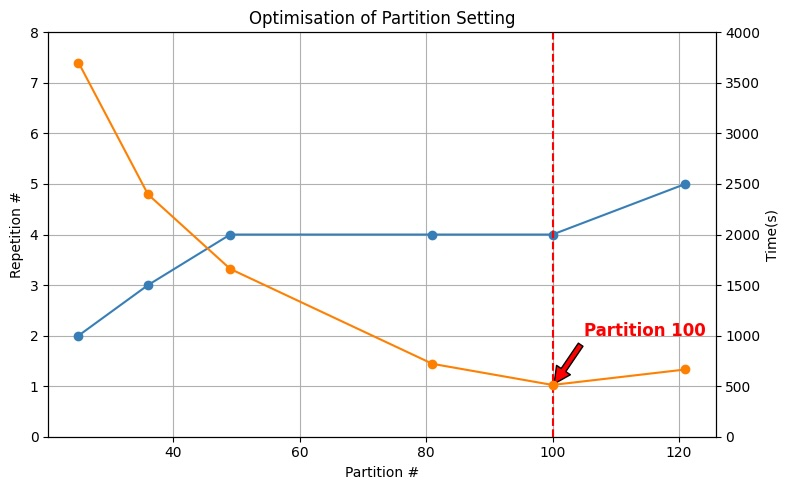
\includegraphics[width=0.8\linewidth]{optimisation.jpg}
\begin{figure}[htbp]
  \centering
  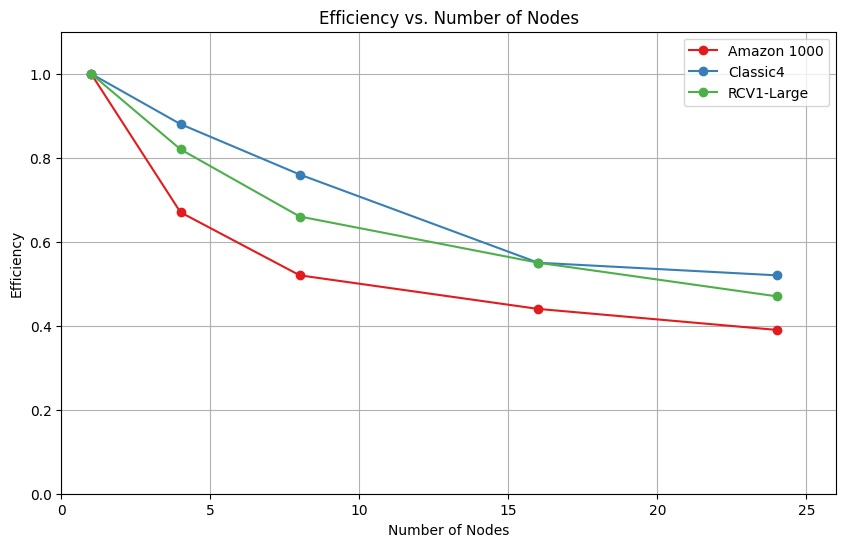
\includegraphics[width=0.8\linewidth]{efficiency.jpg}
  \caption{Enhanced efficiency of the proposed method in handling large-scale datasets.}
  \label{fig:efficiency}
\end{figure}

\Cref{fig:efficiency} presents the efficiency of our proposed co-clustering method across different datasets as the number of nodes increases. The datasets considered are Amazon 1000, Classic4, and RCV1-Large. The x-axis represents the number of nodes, while the y-axis indicates the efficiency, normalized to the baseline (single node) efficiency of 1.

\subsubsection{Amazon 1000 Dataset}
The efficiency starts at 1 for a single node and gradually decreases to 0.39 as the number of nodes increases to 24. The decrease in efficiency is relatively smooth, indicating that our method scales well but exhibits some overhead as more nodes are added. Despite the reduction in efficiency, the method maintains more than 39\% efficiency with 24 nodes, highlighting the robustness of the algorithm even at higher parallelization levels.

\subsubsection{Classic4 Dataset}
The efficiency for Classic4 begins at 1 and decreases to 0.52 with 24 nodes. The drop in efficiency is more pronounced compared to the Amazon 1000 dataset, especially between 4 and 8 nodes, indicating a higher overhead for this dataset as the number of nodes increases. The method still retains more than half of the efficiency at 24 nodes, demonstrating good scalability.

\subsubsection{RCV1-Large Dataset}
Starting from an efficiency of 1, it decreases to 0.47 at 24 nodes. The decrease is relatively smooth, similar to the Amazon 1000 dataset, but with a slightly steeper decline. The method shows a significant efficiency retention at higher node counts, indicating effective parallelization.

\subsection{Detailed Analysis}

\subsubsection{Scalability}
The results demonstrate that our method effectively scales across multiple nodes, maintaining a reasonable level of efficiency even as the number of nodes increases. This is crucial for large-scale data processing, where distributing the computational load is necessary to handle extensive datasets without incurring prohibitive computational costs.

\subsubsection{Dataset Characteristics}
The differences in efficiency reduction between datasets highlight the influence of dataset characteristics on parallelization. For instance, Classic4 shows a more significant drop, which could be due to its specific data structure or inherent complexity that introduces more overhead when partitioned across nodes. The smoother efficiency decline for Amazon 1000 and RCV1-Large suggests that these datasets are more amenable to parallel processing, possibly due to less inter-node communication or better partitioning.

\subsubsection{Parallel Processing Overhead}
The observed decrease in efficiency is expected due to the overhead introduced by parallel processing, such as inter-node communication, synchronization, and data partitioning. Our method's design, which includes dynamic partitioning and hierarchical merging, helps mitigate these overheads to a significant extent, as evidenced by the relatively high efficiency retention.

\subsubsection{Practical Implications}
Maintaining around 40-50\% efficiency with up to 24 nodes is a strong indicator that our method can handle very large datasets in a distributed computing environment effectively. This efficiency retention is critical for real-world applications where computational resources are distributed across many nodes, and maintaining high performance is essential for timely data processing.

\subsection{Optimal Partitioning}

We further analyzed the optimization of partition settings to determine the ideal balance between the number of partitions, the number of repetitions, and the computation time. The datasets were divided into varying numbers of partitions: 25, 36, 49, 81, 100, and 121. For each partition setting, the required number of repetitions and the corresponding computation time (in seconds) were recorded. The experiment aimed to identify the optimal partition setting that minimizes computation time while maintaining a feasible number of repetitions. The results, shown in Figure~\ref{fig:optimisation}, highlight the optimal setting at 100 partitions, where computation time is minimized, and the number of repetitions remains stable.

%include images/efficiency.jpg
\begin{figure}[htbp]
  \centering
  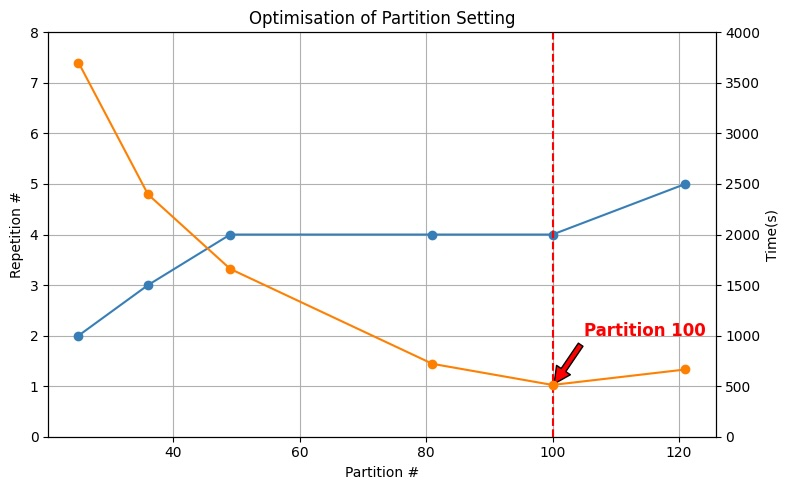
\includegraphics[width=0.8\linewidth]{optimisation.jpg}
  \caption{Optimization of the partitioning algorithm for computational efficiency.}
  \label{fig:optimisation}
\end{figure}

\Cref{fig:optimisation} illustrates the relationship between the number of partitions, the number of repetitions, and the computation time (in seconds). The x-axis represents the number of partitions, while the primary y-axis indicates the number of repetitions, and the secondary y-axis shows the computation time in seconds. The plot provides valuable insights into how our proposed method performs under varying partition settings.

\subsubsection{Repetition Count}
The blue line represents the number of repetitions needed for different partition counts. As the number of partitions increases from 25 to 121, the number of repetitions initially rises, peaking at 4 for partitions 49, 81, and 100 before slightly increasing to 5 at 121 partitions. This trend suggests that more partitions generally require a higher number of repetitions to achieve optimal co-clustering, but there is a point of diminishing returns.

\subsubsection{Computation Time}
The orange line shows the computation time corresponding to different partition counts. There is a noticeable decrease in computation time as the number of partitions increases from 25 to 100, with the time dropping from 3701 seconds to 512 seconds. However, the computation time slightly increases to 665 seconds at 121 partitions. This indicates that while increasing the number of partitions initially improves computational efficiency, beyond a certain point, the overhead of managing more partitions outweighs the benefits.

\subsubsection{Optimal Partition Setting}
The red dashed line at 100 partitions highlights the theoretical optimal setting, where the computation time is minimized. At this setting, the number of repetitions required is stable at 4, and the computation time is at its lowest. This confirms that our theoretical analysis aligns with empirical results, validating the effectiveness of our partitioning strategy.

\subsubsection{Balancing Partitions and Repetitions}
The results indicate that there is an optimal balance between the number of partitions and the number of repetitions required. Too few partitions result in higher computation times due to the increased complexity within each partition, while too many partitions lead to increased overhead from managing numerous small partitions.

\subsubsection{Efficiency and Scalability}
The significant reduction in computation time as the number of partitions increases up to 100 demonstrates the scalability of our method. This efficiency gain is crucial for processing large-scale datasets, where computational resources and time are often limiting factors. The slight increase in computation time beyond 100 partitions suggests that there is an optimal range for partition counts that maximizes efficiency without incurring excessive overhead.

\subsubsection{Practical Implications}
The practical implication of these findings is that our proposed method can be effectively tuned for various datasets by adjusting the number of partitions. The theoretical optimal setting at 100 partitions provides a benchmark for achieving the best performance, but the method's flexibility allows for adjustments based on specific dataset characteristics and computational constraints.

These experiments validated that our Matrix Partitioned and Hierarchical Co-Cluster Merging is an efficient and accurate approach to analyze large data matrices. The method's innovative partitioning strategy and ensemble clustering technique offer a new direction for scalable and precise co-clustering in data analysis.

\section{Conclusion}
\label{sec:conclusion}
This paper presents a novel and scalable co-clustering method for large-scale datasets, leveraging a divide-and-conquer strategy to partition the input matrix into smaller submatrices for parallel processing, thereby significantly reducing computational overhead. Each submatrix is co-clustered independently using a probabilistic model-based optimal partitioning algorithm, ensuring the integrity of co-clusters, and the results are combined using a hierarchical co-cluster merging algorithm to enhance accuracy and reliability. Our implementation using the Message Passing Interface (MPI) distributes the computational load across multiple nodes, improving scalability and making the approach practical for large-scale applications without requiring specialized performance from any single node. Experimental results demonstrate substantial improvements in computational efficiency and scalability, confirming the method's effectiveness for diverse and extensive datasets. This work addresses the challenges of co-clustering large-scale data by integrating efficient partitioning, parallel processing, and robust merging techniques, setting a new benchmark for scalable co-clustering and paving the way for future research in scalable data analysis technologies.


\printbibliography

\end{document}